\iffalse
This file is protected by Copyright. Please refer to the COPYRIGHT file
distributed with this source distribution.

This file is part of OpenCPI <http://www.opencpi.org>

OpenCPI is free software: you can redistribute it and/or modify it under the
terms of the GNU Lesser General Public License as published by the Free Software
Foundation, either version 3 of the License, or (at your option) any later
version.

OpenCPI is distributed in the hope that it will be useful, but WITHOUT ANY
WARRANTY; without even the implied warranty of MERCHANTABILITY or FITNESS FOR A
PARTICULAR PURPOSE. See the GNU Lesser General Public License for more details.

You should have received a copy of the GNU Lesser General Public License along
with this program. If not, see <http://www.gnu.org/licenses/>.
\fi
%----------------------------------------------------------------------------------------
% Update the docTitle and docVersion per document
%----------------------------------------------------------------------------------------
\def\docTitle{Getting Started Guide}
\def\docVersion{1.3}
%----------------------------------------------------------------------------------------
\documentclass{article}
\iffalse
This file is protected by Copyright. Please refer to the COPYRIGHT file
distributed with this source distribution.

This file is part of OpenCPI <http://www.opencpi.org>

OpenCPI is free software: you can redistribute it and/or modify it under the
terms of the GNU Lesser General Public License as published by the Free Software
Foundation, either version 3 of the License, or (at your option) any later
version.

OpenCPI is distributed in the hope that it will be useful, but WITHOUT ANY
WARRANTY; without even the implied warranty of MERCHANTABILITY or FITNESS FOR A
PARTICULAR PURPOSE. See the GNU Lesser General Public License for more details.

You should have received a copy of the GNU Lesser General Public License along
with this program. If not, see <http://www.gnu.org/licenses/>.
\fi
\author{} % Force author to be blank
%----------------------------------------------------------------------------------------
% Paper size, orientation and margins
%----------------------------------------------------------------------------------------
\usepackage{geometry}
\geometry{
        letterpaper, % paper type
        portrait,    % text direction
        left=.75in,  % left margin
        top=.75in,   % top margin
        right=.75in, % right margin
        bottom=.75in % bottom margin
 }
%----------------------------------------------------------------------------------------
% Header/Footer
%----------------------------------------------------------------------------------------
\usepackage{fancyhdr} \pagestyle{fancy} % required for fancy headers
\renewcommand{\headrulewidth}{0.5pt}
\renewcommand{\footrulewidth}{0.5pt}
\rhead{\small{ANGRYVIPER Team}}
% \rfoot{\thepage}
%----------------------------------------------------------------------------------------
% Appendix packages
%----------------------------------------------------------------------------------------
\usepackage[toc,page]{appendix}
%----------------------------------------------------------------------------------------
% Defined Commands & Renamed Commands
%----------------------------------------------------------------------------------------
\renewcommand{\contentsname}{Table of Contents}
\renewcommand{\listfigurename}{List of Figures}
\renewcommand{\listtablename}{List of Tables}
%----------------------------------------------------------------------------------------
% Various packages
%----------------------------------------------------------------------------------------
\usepackage[usenames,dvipsnames]{xcolor} % for color names see https://en.wikibooks.org/wiki/LaTeX/Colors
\usepackage{hyperref}  % for linking urls and lists
\usepackage{graphicx}  % for including pictures by file
\usepackage{listings}  % for coding language styles
\usepackage{rotating}  % for sideways table
\usepackage{pifont}    % for sideways table
\usepackage{pdflscape} % for landscape view
\usepackage{subfig}
\usepackage{xstring}
\uchyph=0 % Never hyphenate acronyms like RCC (I think this overrides ANGRYVIPER above)
\renewcommand\_{\textunderscore\allowbreak} % Allow words to break/newline on underscores
%----------------------------------------------------------------------------------------
% Table packages
%----------------------------------------------------------------------------------------
\usepackage{longtable} % for long possibly multi-page tables
\usepackage{tabularx} % c=center,l=left,r=right,X=fill
% These define tabularx columns "C" and "R" to match "X" but center/right aligned
\newcolumntype{C}{>{\centering\arraybackslash}X}
\newcolumntype{R}{>{\raggedleft\arraybackslash}X}
\usepackage{float}
\floatstyle{plaintop}
\usepackage[tableposition=top]{caption}
\newcolumntype{P}[1]{>{\centering\arraybackslash}p{#1}}
\newcolumntype{M}[1]{>{\centering\arraybackslash}m{#1}}
%----------------------------------------------------------------------------------------
% Block Diagram / FSM Drawings
%----------------------------------------------------------------------------------------
\usepackage{tikz}
\usetikzlibrary{shapes,arrows,fit,positioning}
\usetikzlibrary{automata} % used for the fsm
%----------------------------------------------------------------------------------------
% Colors Used
%----------------------------------------------------------------------------------------
\usepackage{colortbl}
\definecolor{blue}{rgb}{.7,.8,.9}
\definecolor{ceruleanblue}{rgb}{0.16, 0.32, 0.75}
\definecolor{drkgreen}{rgb}{0,0.6,0}
\definecolor{deepmagenta}{rgb}{0.8, 0.0, 0.8}
\definecolor{cyan}{rgb}{0.0,0.6,0.6}
\definecolor{maroon}{rgb}{0.5,0,0}
%----------------------------------------------------------------------------------------
% VHDL Coding Language Style
% modified from: http://latex-community.org/forum/viewtopic.php?f=44&t=22076
%----------------------------------------------------------------------------------------
\lstdefinelanguage{VHDL}
{
        basicstyle=\ttfamily\footnotesize,
        columns=fullflexible,keepspaces,      % https://tex.stackexchange.com/a/46695/87531
        keywordstyle=\color{ceruleanblue},
        commentstyle=\color{drkgreen},
        morekeywords={
    library,use,all,entity,is,port,in,out,end,architecture,of,
    begin,and, signal, when, if, else, process, end,
        },
        morecomment=[l]--
}
%----------------------------------------------------------------------------------------
% XML Coding Language Style
% modified from: http://tex.stackexchange.com/questions/10255/xml-syntax-highlighting
%----------------------------------------------------------------------------------------
\lstdefinelanguage{XML}
{
        basicstyle=\ttfamily\footnotesize,
        columns=fullflexible,keepspaces,
        morestring=[s]{"}{"},
        morecomment=[s]{!--}{--},
        commentstyle=\color{drkgreen},
        moredelim=[s][\color{black}]{>}{<},
        moredelim=[s][\color{cyan}]{\ }{=},
        stringstyle=\color{maroon},
        identifierstyle=\color{ceruleanblue}
}
%----------------------------------------------------------------------------------------
% DIFF Coding Language Style
% modified from http://tex.stackexchange.com/questions/50176/highlighting-a-diff-file
%----------------------------------------------------------------------------------------
\lstdefinelanguage{diff}
{
        basicstyle=\ttfamily\footnotesize,
        columns=fullflexible,keepspaces,
        breaklines=true,                                % wrap text
        morecomment=[f][\color{ceruleanblue}]{@@},      % group identifier
        morecomment=[f][\color{red}]-,                  % deleted lines
        morecomment=[f][\color{drkgreen}]+,             % added lines
        morecomment=[f][\color{deepmagenta}]{---},      % Diff header lines (must appear after +,-)
        morecomment=[f][\color{deepmagenta}]{+++},
}
%----------------------------------------------------------------------------------------
% Python Coding Language Style
% modified from
%----------------------------------------------------------------------------------------
\lstdefinelanguage{python}
{
        basicstyle=\ttfamily\footnotesize,
        columns=fullflexible,keepspaces,
        keywordstyle=\color{ceruleanblue},
        commentstyle=\color{drkgreen},
        stringstyle=\color{orange},
        morekeywords={
    print, if, sys, len, from, import, as, open,close, def, main, for, else, write, read, range,
        },
        comment=[l]{\#}
}
%----------------------------------------------------------------------------------------
% Fontsize Notes in order from smallest to largest
%----------------------------------------------------------------------------------------
%    \tiny
%    \scriptsize
%    \footnotesize
%    \small
%    \normalsize
%    \large
%    \Large
%    \LARGE
%    \huge
%    \Huge

\setlength{\parindent}{0pt} % Don't indent all paragraphs
\newcommand{\forceindent}{\leavevmode{\parindent=1em\indent}}
\date{Version \docVersion} % Force date to be blank and override date with version
\title{\docTitle}
\lhead{\small {\docTitle} }
%----------------------------------------------------------------------------------------
% This makes sure that our verbatim blocks don't get pagebreaks in them
\def\bstart{~\\
\begin{minipage}{\linewidth}}
\def\bend{\end{minipage}
~\\
}
\usepackage{listings}
\usepackage{xcolor}
\usepackage{textcomp}
\begin{document}
\maketitle
\thispagestyle{fancy}
\newpage

        \begin{center}
        \textit{\textbf{Revision History}}
                \begin{table}[H]
                \label{table:revisions} % Add "[H]" to force placement of table
                        \begin{tabularx}{\textwidth}{|c|X|l|}
                        \hline
                        \rowcolor{blue}
                        \textbf{Revision} & \textbf{Description of Change} & \textbf{Date} \\
                        \hline
                        v1.0 & Initial creation & 2/2016 \\
                        \hline
                        v1.1 & Updated for OpenCPI Release 1.1 & 3/2017 \\
			            \hline
                        v1.2 & Updated for OpenCPI Release 1.2 & 8/2017 \\
                        \hline
                        v1.3 & Updated for OpenCPI Release 1.3 & 2/2018 \\
                        \hline
                        \end{tabularx}
                \end{table}
        \end{center}

\newpage

\tableofcontents

\newpage

\listoffigures

\newpage

\listoftables

\newpage

\section{References}

This document assumes a basic understanding of the Linux command line environment. It does not require a working knowledge of OpenCPI.
\def\refskipgs{} % Skip self
\def\myreferences{
% you can add "info" between goo.gl and the tag for analytics
\hline
Component Development Guide & OpenCPI & \url{https://goo.gl/zBwIe0} \\
\hline
RCC Development Guide & OpenCPI & \url{https://goo.gl/0ix1E0} \\
\hline
HDL Development Guide & OpenCPI & \url{https://goo.gl/OVmRhI} \\
}
\iffalse
This file is protected by Copyright. Please refer to the COPYRIGHT file
distributed with this source distribution.

This file is part of OpenCPI <http://www.opencpi.org>

OpenCPI is free software: you can redistribute it and/or modify it under the
terms of the GNU Lesser General Public License as published by the Free Software
Foundation, either version 3 of the License, or (at your option) any later
version.

OpenCPI is distributed in the hope that it will be useful, but WITHOUT ANY
WARRANTY; without even the implied warranty of MERCHANTABILITY or FITNESS FOR A
PARTICULAR PURPOSE. See the GNU Lesser General Public License for more details.

You should have received a copy of the GNU Lesser General Public License along
with this program. If not, see <http://www.gnu.org/licenses/>.
\fi

% This snippet creates the "References" table labeled "table:references"
% It creates three columns: Name, Publisher, Link and then inserts default documents
%
% To skip these defaults, define macros named
% refskipgs to skip "Getting Started"
% refskipig to skip "Installation Guide"
% refskipac to skip "Acronyms and Definitions"
% refskipocpiov to skip "OpenCPI Overview"
%
% See RPM_Installation_Guide.tex for examples
%
% After the defaults, it optionally inserts the "myreferences" macro that
% you defined elsewhere (you put hlines above all lines)
%
% If you want the \caption on the bottom, define "refcapbottom"
\begin{center}
\renewcommand*\footnoterule{} % Remove separator line from footnote
\renewcommand{\thempfootnote}{\arabic{mpfootnote}} % Use Arabic numbers (or can't reuse)
\begin{minipage}{0.9\textwidth}
  \begin{table}[H]
\ifx\refcapbottom\undefined
  \caption {References}
  \label{table:references}
\fi
  \begin{tabularx}{\textwidth}{|C|C|}
    \hline
    \rowcolor{blue}
    \textbf{Title} & \textbf{Link} \\
\ifx\refskipocpiov\undefined
    \hline
    OpenCPI Overview & \githubio{Overview.pdf} \\
\fi
\ifx\refskipac\undefined
    \hline
    Acronyms and Definitions & \githubio{Acronyms\_and\_Definitions.pdf} \\
\fi
\ifx\refskipgs\undefined
    \hline
    Getting Started & \githubio{Getting\_Started.pdf} \\
\fi
\ifx\refskipig\undefined
    \hline
    Installation Guide & \githubio{RPM\_Installation\_Guide.pdf} \\
\fi
\ifx\myreferences\undefined
\else
    \myreferences
\fi
    \hline
  \end{tabularx}
\ifx\refcapbottom\undefined
\else
  \caption {References}
  \label{table:references}
\fi
  \end{table}
\end{minipage}
\end{center}


\newpage
\section{What is the ANGRYVIPER Team?}
\label{sec:what_is_angryviper}
The ANGRYVIPER Team is a group of engineers contracted to support the OpenCPI framework with additional features, reference assets (known as \textbf{\texttt{ocpi.assets}}), additional API, RPM-based modular installation, and an integrated development environment (IDE).

\subsection{Overview of OpenCPI}
Open Component Portability Infrastructure (OpenCPI) is a series of tools and runtime platform for developing and deploying heterogeneous applications. It includes:
\begin{itemize}
\item A runtime environment to manage and deploy assets in both software and HDL.
\item A set of tools for development of applications and components for software and HDL.
\item A framework and methodology for targeting mixed processor architecture types.
\item A set of HDL and software building blocks for developers to use and expand.
\item A series of reference applications running on base platforms.
\end{itemize}

Assets and applications developed using OpenCPI are meant to simplify complex integration and improve code portability of heterogeneous solutions. OpenCPI extends component-based architectures into GPPs and FPGAs to decrease development costs and time to market through code portability, reuse, and ease of integration.

\subsection{Projects Overview}
Historically, all OpenCPI development, for both the core team and the end user, has been within a single directory structure. As the team size and user base expand, this quickly becomes untenable, especially when taking version control systems into account. The previous working area has been broken into several locations. \\

The CDK and the source for the Core and Assets Projects are provided by the ANGRYVIPER Team in the form of various RPMs that can be installed by a System Administrator. A version of the Core Project is provided containing prebuilt software necessary for all OpenCPI execution (and optionally development).  In order to exercise any of the supported FPGA platforms, a user must have a writable copy of the Core project in order to build HDL using his/her own specific FPGA tool version(s).

\begin{center}
\begin{table}[h]
\caption{Project Types}
%\captionof{table}{\text{Project Types}}
\begin{tabularx}{\textwidth}{|c|C|C|}
\hline
\rowcolor{blue}
Name & Contents & Expectation/Usage\\
\hline
CDK & Framework, Utilities & End-user will use, not modified
\\
\hline
Core Project & Minimal Components, Primitives, RCC Platforms, HDL Simulator Platforms & End-user will build, not modify
\\
\hline
Assets Project & Applications, Components, Primitives, Platforms, Cards/Slots, Devices, Assemblies  & End-user will build, run, maybe modify
\\
\hline
BSP Project & Platforms, Cards/Slots, Devices, etc.  & End-user will build, not modify
\\
\hline
User Project & User-provided Components, Applications, etc. & End-user will build, run, modify
\\
\hline
\end{tabularx}
\end{table}
\end{center}

\newpage
\section{A Brief overview OpenCPI's Architecture}
In this section, the basics of the framework are discussed including the communications, control, and data exchange.
\label{sec:brief_ow_arch}
At the highest level, the architecture of the framework is connectivity between three key concepts:
\begin{itemize}
\item \textbf{Application Management Model}: How component-based applications are managed and controlled including loading, launching, starting, stopping, configuring, querying, etc. This is sometimes described as how component-based applications are deployed.
\item \textbf{Authoring Model:} How components are written in order to be effective on various
processing technologies and execution environments.
\item \textbf{Data Transport:} How messages are moved between one component and another.
\end{itemize}

The core software is structured to allow extensions in any of these three dimensions: enable new management models, add new authoring models, and adding new data transport technologies. \newline

Figure~\ref{fig:what_is_av} represents the conceptual plug and play functionality AV brings through the use of extensions. These extension can take the form of management models, new authoring models and new data technologies.

\begin{figure}[h]
\centerline{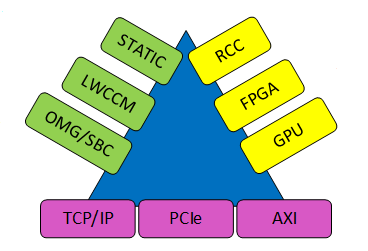
\includegraphics[scale=0.75]{./figures/pillars_of_ocpi.png}}
\caption{Conceptual extensibility of the OpenCPI framework for new and expanding target bases. Reflecting the three key concepts: Application Management, Authoring Model, and Data Transport.}
\label{fig:what_is_av}
\end{figure}

\subsection{Management Models}
\label{subsec:Mangement_models}
The basis for the management model is to specify how applications are managed and deployed, including how a control application would statically or dynamically decide to execute one or more component-based applications on a given system. The framework provides two different modes. The first is an application called \verb+ocpirun+, which takes an application XML and control commands to execute. The second is through the use of native C++ API for controlling and launching applications which gives the application developer a greater level of control, including reading and writing properties during execution.

\subsection{Authoring Models}
\label{subsec:Authoring_Models}
The framework uses the concept of ``containers'' which can host and execute workers. These workers can be hardware-oriented (VHDL within an FPGA) or software-oriented (C/C++ on a GPP\footnote{Standalone or within an FPGA}).
% This is "getting started" not history and background... The architecture of the software base is structured to easily add support of new authoring models for the runtime. This is based on a container plug-in model where container software and HDL can be configured into the system based on the need for supporting specific authoring models on specific processing devices. This can be done either using static or dynamic linking.

\subsection{Data Transport}
\label{subsec:Data_Transport}
The communication model is conceptually based on a protocol model where a component is defined to be able to send or receive messages
with defined payloads. The protocol can be as simple as ``frames of 200 16-bit unsigned integers''. It can also be a variety of messages in a variety of formats based on variable length data types. The transport mechanism can be:
\begin{itemize}
\item Passing buffer pointers with no data copying between collocated workers in software.
\item Directly connecting wires from one FPGA worker to another.
\item Moving messages over network sockets (TCP/IP).
\item Moving messages between processors using standard buses (PCIe or AXI).
\end{itemize}

The benefit here is a flexible and transparent methodology for moving data of differing types from worker to worker. This enables a simplified and abstracted development process that greatly removes the hardware implementation from the application.

\newpage
\section{Getting Started}
This section will walk through building the Base Project and all the fundamental steps of creating, building, running, and testing a simple application containing HDL workers. In the \textit{OpenCPI Component Development Guide}, the \verb+ocpidev+ command line tool is discussed in detail, but this example will serve as an introduction to using the \verb+ocpidev+ command line tool.

\subsection{Installation of OpenCPI}
The most direct method for installation of the OpenCPI framework and IDE is through the use of the OpenCPI RPMs. The RPMs allows for a normalized installation process with the inclusion of all dependencies required. A detailed installation process can be found in the \textit{RPM Installation Guide}.

\begin{center}
\framebox{\parbox{0.8\linewidth}{\centering The remainder of this document assumes the RPMs have been installed. The user's environmental variables must also be configured to build with the Xilinx Vivado software.}}
\end{center}

\subsection{Environmental Variables}
Various environmental variables are used to control OpenCPI. When installed, the RPMs provide ``sane'' defaults for all, and \verb+OCPI_LIBRARY_PATH+ is often the only one an end user will need to modify. However, the ones listed in Table~\ref{table:variables} are often useful for debugging purposes.

	\begin{center}
		\begin{table}[H]
		\caption {Commonly Used Variables}\label{tab:env}
		\label{table:variables}
			\begin{tabularx}{\textwidth}{|c|X|}
\hline
\rowcolor{blue}\textbf{Main RPMs} & \textbf{Description} \\
\hline
\verb+OCPI_CDK_DIR+ &
The location of the CDK's installation. If unset, many scripts and programs will fail to operate. With RPM installation, it is \textit{always} \path{/opt/opencpi/cdk}.\\
\hline
\verb+OCPI_LIBRARY_PATH+ &
The set of locations (or projects) used to find runtime artifacts. \textit{Every file within every path} in this colon-separated list is opened and examined for deployment metadata. For this reason, it is best to point to each projects' \path{exports} subdirectory and not their root location.\\
\hline
\verb+OCPI_LOG_LEVEL+ &
The amount of logging output by the runtime system. The default is zero (\textbf{0}), indicating no logging output. The maximum logging is \textbf{20}. Commonly useful startup and diagnostic information (\textit{e.g.} artifact discovery feedback) is provided at log level \textbf{8}. Unusual events are logged at level \textbf{4}.\\
\hline
\verb+OCPI_PROJECT_PATH+ &
The set of projects used to find various artifacts and support infrastructure \textit{during build time}. This colon-separated list is legacy (but still supported) and largely replaced by the project registry (detailed below).\\
\hline
\verb+OCPI_PROJECT_REGISTRY_DIR+ &
Override the default location of the project registry. If this is not set, the default project registry is OCPI\_CDK\_DIR/../project-registry.\\
\hline
\verb+OCPI_SYSTEM_CONFIG+ &
The runtime system XML configuration file. Default is \path{/opt/opencpi/system.xml} with a fallback to \path{/opt/opencpi/cdk/default-system.xml}.\\
\hline
			\end{tabularx}
		\end{table}
	\end{center}
\subsection{Project Registry}
A project registry is a directory that contains references to projects in a development environment. By registering a project, a user is publishing his project so it can be referenced/searched by any user or project using that same project registry. The default project registry is explained in the OCPI\_PROJECT\_REGISTRY\_DIR row of in table \ref{tab:env}. \\

To add a project to the default project registry, a user needs to be in the \code{opencpi} user group.  This is described in detail the \textit{RPM Installation Guide}.  The \verb+ocpidev register project+ command is used to register a project. This is done automatically when the first copies of the core and assets projects are created. For user-provided projects (or new copies/overrides of the core/assets projects), the \code{register} command can be used. \code{unregister} can be used to remove an existing project from the registry. \footnote{Note that \code{unregister} does not remove your project, it just delists it from the registry}

The project registry can also be set on a per-project basis using \code{ocpidev set registry <registry-location>}. See \code{ocpidev --help set} for more information.

\subsection{Create and Build the Core and Assets Project}
\subsubsection{Create Core}
With the \texttt{opencpi-devel} rpm installed, a \texttt{core} project can be created. It is recommended that each user has his/her own copy of the \texttt{core} project. Included with the CDK is an installation script, \path{/opt/opencpi/projects/new_project_source} . This script will copy the read-only \texttt{core} project out of \path{/opt/opencpi/projects/core} and into another location. The script takes two parameters: the project being copied and the destination folder, \verb+~/ocpi_coreproject+ is the recommended location. Before running this script, make sure the user is a member of the \code{opencpi} group as explained in the \textit{RPM Installation Guide}.\\

\verb+% /opt/opencpi/projects/new_project_source core <path>/<name>+\\

This command may produce a handful of warnings. It is likely that these warnings can be ignored. If the command actually outputs an Error, it is likely because the user is not a member of the \code{opencpi} group.

\subsubsection{Create Assets}
With the \texttt{opencpi-project-assets} RPM present, a copy of the \texttt{assets} project can be installed. It is recommended that each user has his/her own copy of \texttt{assets}. Included with the CDK is an installation script, \path{/opt/opencpi/projects/new_project_source} . This script will copy the template \texttt{assets} project out of \path{/opt/opencpi/projects/assets} and into another location. The script takes two parameters the project being copied and the destination folder, \verb+~/ocpi_assetsproject+ is the recommended location.\\

\verb+% /opt/opencpi/projects/new_project_source assets <path>/<name>+

\subsubsection{Display Installed Projects}
To confirm which projects are installed and where they live, the command \texttt{ocpidev show projects --table} can be used.
\subsubsection{Building Projects}
\label{subsubsec:buildworkers}
In this step, the Project's contents will be built. Before completing the remaining steps, the environment must be set up as described in the \textit{RPM Installation Guide}.\\

To build a project, first pick the desired \textit{Platform} to build for. The available options are listed in Table~\ref{table:hdlworkers}.

	\begin{center}
		\renewcommand*\footnoterule{} % Remove separator line from footnote
		\renewcommand{\thempfootnote}{\arabic{mpfootnote}} % Use Arabic numbers (or can't reuse)
		\begin{minipage}{.623\textwidth}
		\begin{table}[H]
		\caption {Supported Platforms}\label{tab:plats}
		\label{table:hdlworkers} % Add "[H]" to force placement of table
			\begin{tabularx}{\textwidth}{|l|l|l|}
			\hline
			\rowcolor{blue}
			\textbf{Simulator Vendor} & \textbf{Platform Name} & \textbf{Project}\\

			\hline
			ModelSim DE 10.6a/10.4c & \code{modelsim} & \code{ocpi.core}\\
			\hline
			Xilinx Vivado 2017.1 & \code{xsim} & \code{ocpi.core}\\
			\hline
			Xilinx ISE 14.7 & \code{isim} & \code{ocpi.core}\\
			\hline
			\rowcolor{blue}
			\textbf{Hardware Platform} & \textbf{Platform Name} & \textbf{Project}\\
			\hline
			Epiq Solutions Matchstiq-Z1 & \code{matchstiq\_z1}\footnote{Reference the Matchstiq-Z1 Getting Started Guide to build for \code{matchstiq\_z1}} & \code{ocpi.assets}\\
			\hline
			Avnet ZedBoard & \code{zed}\footnote{Reference the Zedboard Getting Started Guide to build for \code{zedboard}} & \code{ocpi.assets}\\
			\hline
			Avnet ZedBoard (ISE mode) & \code{zed\_ise}\footnote{Use Xilinx ISE tools to build for this platform} & \code{ocpi.assets}\\
			\hline
			Altera Stratix IV GX & \code{alst4} & \code{ocpi.assets}\\
			\hline
			Xilinx ML605 (Virtex-6) & \code{ml605} & \code{ocpi.assets}\\
			\hline
			\rowcolor{blue}
			\textbf{Software Platform} & \textbf{Platform Name} & \textbf{Project}\\
			\hline
			Centos6 & \code{centos6} & \code{ocpi.core}\\
			\hline
			Centos7 & \code{centos7} & \code{ocpi.core}\\
			\hline
			Xilinx Linux (2013 3rd Quarter) & \code{xilinx13\_3}\footnote{RCC platform asociated with the zedboard and matchstiq\_z1 platforms} & \code{ocpi.core}\\
			\hline
% AV-2881 - Removing picoflexor because it is a SW platform in a HW context
%			DRS Picoflexor T6A:S1 & \code{picoflexor}\footnote{reference the Picoflexor Getting Started Guide to build for \code{picoflexor} \\\indent{\indent{(Picoflexor support is \textit{RCC only} at this time)}}}\\
%			\hline
			\end{tabularx}
		\end{table}
		\end{minipage}
	\end{center}

\subsubsection{Build Core Project}
This section presents a handful of commands that can be used to build for various platforms. To complete this Guide using the \code{xsim} simulator, use the build command in the box at the end of this section. \\

Note that all build commands in this Guide can optionally be performed using the ANGRYVIPER IDE instead of ``\code{ocpidev build}''.\\

To build the RCC workers, go to the \texttt{core} project and run:\\ \\
\# If user will later target the Zedboard or Matchstiq-Z1:\\
\code{\% ocpidev build -\--rcc -\--rcc-platform xilinx13\_3 }\\

\# If user will later target the Zedboard and/or Centos7:\\
\code{\% ocpidev build -\--rcc -\--rcc-platform xilinx13\_3 -\--rcc-platform centos7}\\

The \texttt{--rcc-platform} option specifies the RCC platform to the build for.\\

Use the following \verb+ocpidev+ command to build the project for the desired platform using the information from Table~\ref{table:hdlworkers}.\\

\code{\% ocpidev build --rcc-platform <platform name> --hdl-platform <platform name>} \\

Building for multiple platforms can be combined into a single \texttt{ocpidev} call, \textit{e.g.}:\\

\code{\% ocpidev build --hdl-platform modelsim --hdl-platform xsim --hdl-platform isim --rcc-platform centos7 --rcc-platform xilinx13\_3} \\

In the \texttt{core} project, the last operation this command performs is to build the project's \texttt{hdl platforms}. You can be sure it succeeded if the last few sections of output are ``\texttt{=======Building platform xsim}''.\\
\begin{center}
\framebox{\parbox{0.8\linewidth}{\centering For the example in Section~\ref{sec:basic_example}, you \textit{must} build for \texttt{xsim} at a minimum. This takes approximately 10 minutes:\newline

\code{ocpidev build --hdl-platform xsim} \newline

\footnotesize{\textit{Note: }If you have ISE installed instead of Vivado, you can follow this guide using \code{isim} instead of \code{xsim}}
}}
\end{center}


\subsubsection{Build Assets Project}
Refer to table \ref{tab:plats} to determine whether the platform being built for lives in the \code{ocpi.assets} project. If so, follow the same building procedures documented in Section~\ref{subsubsec:buildworkers} for the same platforms. The last assets built in the \texttt{assets} project are \texttt{applications}. You can be sure it succeeded if the last few sections of output include ``\texttt{========Building apps cic\_int\_dc\_offset\_iq\_imbalance\_mixer\_cic\_dec}''.\\

If the \code{xsim} platform is being used, the \code{ocpi.assets} project does \textit{not} need to be built at this time.\\

\newpage
\section{Basic Example Application}
\label{sec:basic_example}
This simple application will contain three HDL Workers: \verb+ramp+, \verb+square+, and \verb+ander+, which can be seen in Figure~\ref{fig:simple_app_diagram}. \newline

\begin{figure}[h]
        \centering
        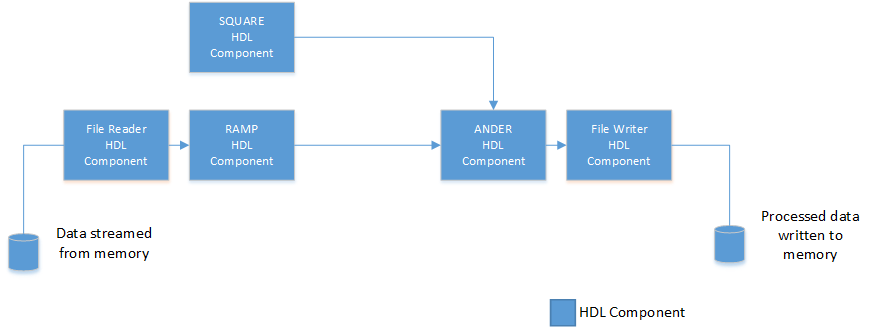
\includegraphics[scale=0.5]{./figures/simple_app_block_diagram.png}
        \caption{Block diagram of simple HDL application with three user-defined workers, a \code{FileRead}, and a \code{FileWrite}.}
        \label{fig:simple_app_diagram}
\end{figure}
For testing and simulation purposes, the OpenCPI \verb+file_read+ and \verb+file_write+ workers will be used to read input data from, and write output data to, files on the system.\newline

The basic format of an \verb+ocpidev+ command is ``\verb+ocpidev [options] <verb> <noun> <name>+''. For this demonstration, the following \verb+nouns+ will be used: \verb+project+, \verb+library+, \verb+spec+, \verb+worker+, \verb+hdl assembly+, and \verb+application+.\newline

The full list of \verb+ocpidev+ verbs, nouns and options can be explored via \code{ocpidev --help}, \code{ocpidev --help <verb>}, or the \textit{OpenCPI Component Development Guide}.

\subsection{Create a Project}
Choose the name ``DemoProject'' for this project. To create the ``DemoProject'' project use the following \verb+ocpidev+ command:\\

\forceindent\verb+% ocpidev create project --register DemoProject+\\

The project that was just created should have also been registered. This assumes the default registry is being used \textit{and} the user is a member of the \code{opencpi} group (as explained in the \textit{RPM Installation Guide}. The project registration can be done separately using the following \verb+ocpidev+ command from within the project:\\

\forceindent\forceindent\verb+% ocpidev register project+\\

Observe the directory structure created, as well as the files.\\

\bstart
\begin{verbatim}
$ tree --charset ascii DemoProject
|-- exports
|   |-- imports -> ../imports
|   `-- project-package-id
|-- imports -> /opt/opencpi/project-registry
|-- Makefile
|-- Project.exports
|-- Project.mk
`-- project.xml
3 directories, 5 files
\end{verbatim}
\bend
Change directories into ``DemoProject''.

\subsection{Create a Library}
A library is a convenient way of grouping workers. For a simple case, the framework defaults to a \verb+components+ directory as the library. To create the default ``components'' library, use the following \verb+ocpidev+ command:\\

\forceindent\verb+% ocpidev create library components+\\

\bstart
Observe the directory structure created, as well as the files:
\begin{verbatim}
DemoProject
|-- components
|   |-- lib
|   |   |-- package-id
|   |   `-- workers
|   |-- Library.mk
|   `-- Makefile
|-- exports
|   |-- imports -> ../imports
|   `-- project-package-id
|-- imports -> /opt/opencpi/project-registry
|-- Makefile
|-- Project.exports
|-- Project.mk
`-- project.xml

\end{verbatim}
\bend
For more advanced projects, one or more libraries would be placed within the \verb+components+ directory. This usage is highly recommended and explained in the \textit{OpenCPI Component Development Guide}.

\subsection{Create Components}
\textit{Components} are black boxes that dictate what properties and interfaces are implemented. A single implementation of a \textit{component} is referred to as a \textit{worker}, which is discussed in the next section. \textit{Components} are defined by an OpenCPI Component Specification (OCS). The OCS is commonly referred to as the \textit{spec file} or \textit{spec}. Each \textit{spec} includes the details that are to be \textbf{consistent among different authoring models}; meaning that if there are various implementations of a single \textit{component}, \textit{e.g.} a software (RCC) worker and an HDL worker, both \textit{workers} expect the same input and both should have the same output regardless of which architecture the worker runs on.\newline

This application requires three \textit{components}, so three \textit{specs} will be generated. To create the three template \textit{specs} use the following \verb+ocpidev+ commands:\\

\forceindent\verb+% ocpidev create spec ramp+

\forceindent\verb+% ocpidev create spec square+

\forceindent\verb+% ocpidev create spec ander+\\
\bstart
\begin{verbatim}
DemoProject
|-- components
|   |-- lib
|   |   |-- package-id
|   |   `-- workers
|   |-- Library.mk
|   |-- Makefile
|   `-- specs
|       |-- ander-spec.xml
|       |-- ramp-spec.xml
|       `-- square-spec.xml
|-- exports
|   |-- imports -> ../imports
|   `-- project-package-id
|-- imports -> /opt/opencpi/project-registry
|-- Makefile
|-- Project.exports
|-- Project.mk
`-- project
\end{verbatim}
\bend
Notice that three \textit{spec} templates were generated. Also note that \textit{spec files} can be easily identified by their \verb+-spec+ postfix\footnote{Some older spec files use \texttt{\_spec} as well.}. In between the \verb+ComponentSpec+ XML tags, the \textit{component} properties and interfaces need to be defined. \textbf{Every component interface (or \textit{port}) must define the direction and format of the messages they will send or receive.} This formatting is known as the \textit{protocol}, and for this example, we will use \texttt{rstream}, which is a stream of up to 4096 16-bit samples per message.

\bstart
For the \verb+ramp+ \textit{component}, insert the following XML snippet in between the \verb+ComponentSpec+ XML tags:

\begin{lstlisting}[language=xml]
<Port Name="in" Producer="false" Protocol="rstream_protocol.xml"/>
<Port Name="out" Producer="true" Protocol="rstream_protocol.xml"/>
\end{lstlisting}
\bend
\bstart
For the \verb+square+ \textit{component}, insert the following XML snippet in between the \verb+ComponentSpec+ XML tags:

\begin{lstlisting}[language=xml]
<Property Name="messagesize" Type="ushort" Default="2048" Readable="true" Writable="true"/>
<Port Name="out" Producer="true" Protocol="rstream_protocol.xml"/>
\end{lstlisting}
\bend
\bstart
For the \verb+ander+ \textit{component}, insert the following XML snippet in between the \verb+ComponentSpec+ XML tags:

\begin{lstlisting}[language=xml]
<Port Name="in1" Producer="false" Protocol="rstream_protocol.xml"/>
<Port Name="in2" Producer="false" Protocol="rstream_protocol.xml"/>
<Port Name="out" Producer="true" Protocol="iqstream_protocol.xml"/>
\end{lstlisting}
\bend
For more details, see the \textit{OpenCPI Component Development Guide}. Now that the \textit{specs} are defined, the next step is to create the \textit{workers}.

\subsection{Create Workers}
As mentioned in the previous section, \textit{workers} are specific implementations of \textit{components}. More than one \textit{worker} can implement a \textit{component}. For this example, only one implementation per \textit{component} will be used, and each of these \textit{workers} are \textit{HDL Workers}. More details about \textit{HDL Workers} can be found in the \textit{OpenCPI HDL Development Guide}. This example does not use any \textit{RCC Workers}, but more details about them can be found in the \textit{OpenCPI RCC Development Guide}.\newline

When creating \textit{workers}, two options need to be defined, one implicitly and one explicitly. The type of \textit{worker} is defined implicitly by appending either \verb+.rcc+ or \verb+.hdl+ to the name of the \textit{worker}. \textit{HDL Workers} use the general format for the \textit{worker} names: \verb+worker_name.hdl+. The language of the \textit{worker} can be explicitly defined; for \textit{RCC Workers} there are currently two choices: C or C++.\newline

To create the \textit{HDL Workers}, use the following \verb+ocpidev+ commands:\\

\forceindent\verb+% ocpidev create worker ramp.hdl+

\forceindent\verb+% ocpidev create worker square.hdl+

\forceindent\verb+% ocpidev create worker ander.hdl+\\

Notice that the creation of the \verb+ramp+, \verb+square+, and \verb+ander+ \textit{HDL Workers} generated a \verb+.hdl+ directory for each. Each of the \verb+.hdl+ directories contain that \textit{worker}'s \textit{OpenCPI Worker Description} (OWD), which can be identified by the following format: \verb+worker_name.xml+. The OWD is where that \textit{worker's} specific properties and port protocols are defined. The definitions in the OWD are specific to each individual worker and may override a set of attributes defined in the OCS. Later the OWD will be edited for each \textit{worker}.\newline

Observe that in each of the \verb+.hdl+ directories there is also the \textit{skeleton file} or \textit{wrapper} in the language that was specified. In this case, the \verb+worker_name.vhd+ is the \textit{skeleton file} for the language option VHDL. Later, the \textit{skeleton file} will be edited for each \textit{worker}.\newline

The \verb+gen+ directory contains other important code that is generated from the framework and will not need to be edited. For more details see the \textit{OpenCPI Component Guide}.\\

\bstart
The project should now look similar to the following:
\begin{verbatim}
DemoProject/
|-- components
|   |-- ander.hdl
|   |   |-- ander.vhd
|   |   |-- ander.xml
|   |   |-- gen
|   |   |   |-- ander-build.xml
|   |   |   |-- ander-defs.vhd
|   |   |   |-- ander-defs.vhd.deps
|   |   |   |-- ander-impl.vhd
|   |   |   |-- ander-impl.vhd.deps
|   |   |   |-- ander.mk
|   |   |   |-- ander-skel.vhd
|   |   |   `-- ander-skel.vhd.deps
|   |   `-- Makefile
|   |-- lib
|   |   |-- hdl
|   |   |   |-- ander-build.xml -> ../../ander.hdl/gen/ander-build.xml
|   |   |   |-- ander.xml -> ../../ander.hdl/ander.xml
|   |   |   |-- ramp-build.xml -> ../../ramp.hdl/gen/ramp-build.xml
|   |   |   |-- ramp.xml -> ../../ramp.hdl/ramp.xml
|   |   |   |-- square-build.xml -> ../../square.hdl/gen/square-build.xml
|   |   |   `-- square.xml -> ../../square.hdl/square.xml
|   |   |-- package-id
|   |   `-- workers
...
|   |-- ramp.hdl
|   |   |-- gen
|   |   |   |-- ramp-build.xml
|   |   |   |-- ramp-defs.vhd
|   |   |   |-- ramp-defs.vhd.deps
|   |   |   |-- ramp-impl.vhd
|   |   |   |-- ramp-impl.vhd.deps
|   |   |   |-- ramp.mk
|   |   |   |-- ramp-skel.vhd
|   |   |   `-- ramp-skel.vhd.deps
|   |   |-- Makefile
|   |   |-- ramp.vhd
|   |   `-- ramp.xml
|   |-- specs
|   |   |-- ander-spec.xml
|   |   |-- ramp-spec.xml
|   |   `-- square-spec.xml
|   `-- square.hdl
|       |-- gen
|       |   |-- square-build.xml
|       |   |-- square-defs.vhd
|       |   |-- square-defs.vhd.deps
|       |   |-- square-impl.vhd
|       |   |-- square-impl.vhd.deps
|       |   |-- square.mk
|       |   |-- square-skel.vhd
|       |   `-- square-skel.vhd.deps
|       |-- Makefile
|       |-- square.vhd
|       `-- square.xml
...
\end{verbatim}
\bend
\bstart
However, if you are using version control, you can determine the key files:
\\\\
First, navigate to the directory above DemoProject
\begin{verbatim}
% ocpidev clean project DemoProject
% tree --charset ascii DemoProject/
DemoProject/
|-- components
|   |-- ander.hdl
|   |   |-- ander.xml
|   |   `-- Makefile
|   |-- Library.mk
|   |-- Makefile
|   |-- ramp.hdl
|   |   |-- Makefile
|   |   `-- ramp.xml
|   |-- specs
|   |   |-- ander-spec.xml
|   |   |-- ramp-spec.xml
|   |   `-- square-spec.xml
|   `-- square.hdl
|       |-- Makefile
|       `-- square.xml
|-- Makefile
|-- Project.exports
|-- Project.mk
`-- project.xml


5 directories, 15 files
\end{verbatim}
\bend

Now the OWD files for each \textit{worker} will be updated. This will provide implementation-specific information for the interfaces that were abstractly defined at the \textit{component} level in the OCS.\\
\bstart
For the \verb+ramp+ \textit{worker}, insert the following in between the \verb+HdlWorker+ XML tags (in \path{components/ramp.hdl/ramp.xml}):

\begin{lstlisting}[language=xml]
<StreamInterface Name="in" DataWidth="16"/>
<StreamInterface Name="out" DataWidth="16"/>
\end{lstlisting}
\bend
\bstart
For the \verb+square+ \textit{worker}, insert the following in between the \verb+HdlWorker+ XML tags (in \path{components/square.hdl/square.xml}):

\begin{lstlisting}[language=xml]
<StreamInterface Name="out" DataWidth="16"/>
\end{lstlisting}
\bend
\bstart
For the \verb+ander+ \textit{worker}, insert the following in between the \verb+HdlWorker+ XML tags (in \path{components/ander.hdl/ander.xml}):

\begin{lstlisting}[language=xml]
<StreamInterface Name="in1" DataWidth="16"/>
<StreamInterface Name="in2" DataWidth="16"/>
<StreamInterface Name="out" DataWidth="32"/>
\end{lstlisting}
\bend

For more details, see the \textit{OpenCPI Component Development Guide}. Now that the OWDs are defined, the next step is to edit the VHDL \textit{skeleton files}.

\bstart
At this point, if you did the ``\texttt{ocpidev clean}'' example above, you need to regenerate the example code:
\begin{itemize}
\setlength\itemsep{0pt}
\item \texttt{ocpidev build worker ramp.hdl}
\item \texttt{ocpidev build worker square.hdl}
\item \texttt{ocpidev build worker ander.hdl}
\end{itemize}
\bend
% From here on, we can't force ALL the source to stick to a single page. Instead, we force the signal listings to stay together and suggest that the intro sentence of the next should stay adjacent by weakly suggesting a pagebreak right before it.
\bstart
For the \verb+ramp.vhd+ \textit{skeleton file} (\path{components/ramp.hdl/ramp.vhd}), insert the following \textit{before} the ``begin'':
\begin{lstlisting}[language=vhdl, columns=fullflexible, breaklines=true, prebreak=\textbackslash, basicstyle=\ttfamily, showstringspaces=false, upquote=true]
  signal idata_vld : bool_t;
  signal odata_vld : bool_t;
  signal buff_data : std_logic_vector(15 downto 0);
\end{lstlisting}
\bend
\pagebreak[1]
Replace the content between \code{begin} and \code{end rtl;} with the following:

\begin{lstlisting}[language=vhdl, columns=fullflexible, breaklines=true, prebreak=\textbackslash, basicstyle=\ttfamily, showstringspaces=false, upquote=true]
  -----------------------------------------------------------------------------
  -- Valid Input (when up/downstream Workers ready and upstream is valid
  -----------------------------------------------------------------------------
  idata_vld <= ctl_in.is_operating and in_in.ready and out_in.ready and in_in.valid;
  -----------------------------------------------------------------------------
  -- Take (when upstream Workers ready and valid)
  -----------------------------------------------------------------------------
  in_out.take <= ctl_in.is_operating and in_in.ready and in_in.valid and out_in.ready;
  -----------------------------------------------------------------------------
  -- Valid Output (when "Give")
  -----------------------------------------------------------------------------
  out_out.valid <= odata_vld;

  ramp : process(ctl_in.clk)
  begin
    if rising_edge(ctl_in.clk) then
      if (ctl_in.reset = '1') then
        buff_data <= (others => '0');
        odata_vld <= '0';
      elsif (idata_vld = '1') then
        buff_data <= std_logic_vector(signed(in_in.data) + signed(buff_data));
        odata_vld <= '1';
      else
        odata_vld <= '0';
      end if;
    end if;
  end process ramp;

  out_out.data <= buff_data;
  -----------------------------------------------------------------------------
  -- Give (when downstream Workers ready & valid)
  -----------------------------------------------------------------------------
  out_out.give <= out_in.ready and odata_vld and ctl_in.is_operating;
  -----------------------------------------------------------------------------
  -- Pass the SOM/EOM out
  -----------------------------------------------------------------------------
  out_out.som <= in_in.som;
  out_out.eom <= in_in.eom;
\end{lstlisting}

\bstart
For the \verb+square.vhd+ \textit{skeleton file} (\path{components/square.hdl/square.vhd}), insert the following \textit{before} the ``begin'':
\begin{lstlisting}[language=vhdl, columns=fullflexible, breaklines=true, prebreak=\textbackslash, basicstyle=\ttfamily, showstringspaces=false, upquote=true]
  signal msg_cnt          : unsigned(15 downto 0);
  signal cnt              : unsigned(15 downto 0);
  signal odata_vld        : bool_t;
  signal missed_odata_vld : bool_t := '0';
  signal max_sample_cnt   : unsigned(15 downto 0);
\end{lstlisting}
\bend
\pagebreak[1]
Replace the content between \code{begin} and \code{end rtl;} with the following:

\begin{lstlisting}[language=vhdl, columns=fullflexible, breaklines=true, prebreak=\textbackslash, basicstyle=\ttfamily, showstringspaces=false, upquote=true]
  -----------------------------------------------------------------------------
  -- Simple counter to trigger the square pulse ON and OFF
  -----------------------------------------------------------------------------
  counter : process (ctl_in.clk)
  begin
    if rising_edge(ctl_in.clk) then
      if (ctl_in.reset = '1' or cnt = 63) then
        cnt <= (others => '0');
      elsif (out_in.ready and ctl_in.is_operating) then
        cnt <= cnt + 1;
      end if;
    end if;
  end process counter;
  -----------------------------------------------------------------------------
  -- Generate the square pulse
  -----------------------------------------------------------------------------
  square : process(ctl_in.clk)
  begin
    if rising_edge(ctl_in.clk) then
      if (ctl_in.reset = '1') then
        out_out.data <= (others => '0');
        odata_vld <= '0';
      elsif (out_in.ready and ctl_in.is_operating) then
        if (cnt < 32) then
          out_out.data <= (others => '1');
        else
          out_out.data <= (others => '0');
        end if;
        odata_vld <= '1';
      else
        odata_vld <= '0';
      end if;
    end if;
  end process square;
  -----------------------------------------------------------------------------
  -- Give (when downstream Worker ready & valid)
  -----------------------------------------------------------------------------
  out_out.give <= out_in.ready and (odata_vld or missed_odata_vld) and ctl_in.is_operating;
  -----------------------------------------------------------------------------
  -- Valid Output (when "Give")
  -----------------------------------------------------------------------------
  out_out.valid <= out_in.ready and (odata_vld or missed_odata_vld) and ctl_in.is_operating;
  -----------------------------------------------------------------------------
  -- SOM/EOM - counter set to message size, increment while giving
  -----------------------------------------------------------------------------
  max_sample_cnt <= props_in.messageSize srl 2;

  messageSize_count : process (ctl_in.clk)
  begin
    if rising_edge(ctl_in.clk) then
      if(ctl_in.reset = '1') then
        msg_cnt <= (others => '0');
      elsif (odata_vld = '1') then
        if(msg_cnt = unsigned(std_logic_vector(max_sample_cnt-1))) then
          msg_cnt <= (others => '0');
        else
          msg_cnt <= msg_cnt + 1;
        end if;
      end if;
    end if;
  end process messageSize_count;

  backPressure : process (ctl_in.clk)
  begin
    if rising_edge(ctl_in.clk) then
      if(ctl_in.reset = '1' or out_in.ready = '1') then
        missed_odata_vld <= '0';
      elsif (out_in.ready = '0' and odata_vld = '1') then
        missed_odata_vld <= '1';
      end if;
      out_out.byte_enable <= (others => '1');
    end if;
  end process backPressure;

  -----------------------------------------------------------------------------
  -- SOM Output (when downstream Worker ready, valid and message count is zero)
  -----------------------------------------------------------------------------
  out_out.som <= '1' when (out_in.ready = '1' and odata_vld = '1' and
                           msg_cnt = 0) else '0';
  -----------------------------------------------------------------------------
  -- EOM Output (when downstream Worker is ready, valid and
  -- message count is equal to message length - 1)
  -----------------------------------------------------------------------------
  out_out.eom <= '1' when (out_in.ready = '1' and odata_vld = '1' and
                           msg_cnt = max_sample_cnt-1) else '0';
\end{lstlisting}
\bstart
For the \verb+ander.vhd+ \textit{skeleton file}  (\path{components/ander.hdl/ander.vhd}), insert the following \textit{before} the ``begin'':

\begin{lstlisting}[language=vhdl, columns=fullflexible, breaklines=true, prebreak=\textbackslash, basicstyle=\ttfamily, showstringspaces=false, upquote=true]
  signal idata_vld : bool_t;
  signal odata_vld : bool_t;
\end{lstlisting}
\bend
\pagebreak[1]
Replace the content between \code{begin} and \code{end rtl;} with the following:
\begin{lstlisting}[language=vhdl, columns=fullflexible, breaklines=true, prebreak=\textbackslash, basicstyle=\ttfamily, showstringspaces=false, upquote=true]
  -----------------------------------------------------------------------------
  -- Take (when both upstream Workers and downstream Worker ready)
  -----------------------------------------------------------------------------
  in1_out.take <= in1_in.ready and in2_in.ready and ctl_in.is_operating and out_in.ready;
  in2_out.take <= in1_in.ready and in2_in.ready and ctl_in.is_operating and out_in.ready;

  idata_vld <= ctl_in.is_operating and out_in.ready and
               in1_in.ready and in2_in.ready and
               in1_in.valid and in2_in.valid;
  -----------------------------------------------------------------------------
  -- Enable all bytes on the stream
  -----------------------------------------------------------------------------
  out_out.byte_enable <= (others => '1');
  -----------------------------------------------------------------------------
  -- Data
  -- AND the RAMP and SQUARE pulse together on the lower 16-bits
  -- Let the RAMP data pass through on the upper 16-bits
  -----------------------------------------------------------------------------
  and_low_pass_high : process (ctl_in.clk)
  begin
    if rising_edge(ctl_in.clk) then
      if (ctl_in.reset = '1') then
        out_out.data <= (others => '0');
      elsif (idata_vld = '1') then
        out_out.data(15 downto 0) <= in1_in.data and in2_in.data;
        out_out.data(31 downto 16) <= in1_in.data;
      end if;
      odata_vld <= idata_vld;
      -----------------------------------------------------------------------------
      -- Pass the RAMP's SOM/EOM out
      -----------------------------------------------------------------------------
      out_out.som <= in1_in.som;
      out_out.eom <= in1_in.eom;
    end if;
  end process and_low_pass_high;

  -----------------------------------------------------------------------------
  -- Valid Output (when output data is valid (which includes upstream==ready))
  -----------------------------------------------------------------------------
  out_out.valid <= odata_vld;
  -----------------------------------------------------------------------------
  -- Give (when downstream Workers ready and our output data is valid)
  -----------------------------------------------------------------------------
  out_out.give <= odata_vld and ctl_in.is_operating and out_in.ready;
\end{lstlisting}
The \textit{workers} must be built at this time using the following \verb+ocpidev+ command from the \verb+DemoProject+ directory:\\

\forceindent\verb+% ocpidev build --hdl-platform xsim+

\subsection{Create an HDL Assembly}
Before an application can be made, an \textit{assembly} for the \textit{HDL workers} need to be created. An \textit{HDL assembly} is a synthesized netlist of connected application workers. For this example, use \verb+demo_assembly+ as the name of the assemblies directory for the application. From the \verb+DemoProject+ directory, run the following \verb+ocpidev+ command to create the assembly:\\

\forceindent\verb+% ocpidev create hdl assembly demo_assembly+\\
\bstart
Notice that this command produces the \verb+hdl+ directory, \verb+assemblies+ directory within it, \verb+demo_assembly+ directory within that, and the \textit{OpenCPI HDL Assembly} (OHAD) (\verb+demo_assembly.xml+).

\begin{verbatim}
DemoProject/hdl/
|-- assemblies
|   |-- demo_assembly
|   |   |-- demo_assembly.xml
|   |   `-- Makefile
|   `-- Makefile
`-- Makefile
\end{verbatim}
\bend
\pagebreak[1]
~\\
Navigate to the \verb+demo_assembly+ directory and replace \verb+demo_assembly.xml+ with this XML:
\begin{lstlisting}[language=xml]
<HdlAssembly>
  <Instance Worker="file_read" Connect="ramp"/>
  <Instance Worker="ramp"/>
  <Instance Worker="square"/>
  <Instance Worker="ander" Connect="file_write"/>
  <Instance Worker="file_write"/>
  <Connection>
    <Port Instance="ramp" Name="out"/>
    <Port Instance="ander" Name="in1"/>
  </Connection>
  <Connection>
    <Port Instance="square" Name="out"/>
    <Port Instance="ander" Name="in2"/>
  </Connection>
</HdlAssembly>
\end{lstlisting}
~\\
Now the assembly for this application is complete. To build the HDL assembly, run the following command:\\

\forceindent\verb+% ocpidev build --hdl-platform xsim+\\

This will take a couple of minutes to run. You can confirm that it succeeded by locating the \texttt{*.bitz} file in \path{hdl/assemblies/demo_assembly/container-demo_assembly_xsim_base/target-xsim/}.\\
\subsection{Create an Application}
One of the simplest ways to make an application is to use the \verb+-X+ option of \verb+ocpidev+. This flag will create a simple \textit{OpenCPI Application Specification} (OAS) in the \verb+applications+ directory. In this case, it will also create the \verb+applications+ directory, since it does not yet exist. For the example, choose the name \verb+DemoApp+ for the name of the application. Run the following \verb+ocpidev+ command from the \verb+DemoProject+ directory to generate the application:\\

\forceindent\verb+% ocpidev -X create application DemoApp+\\

Notice that this command generated the applications directory as well as the \verb+DemoApp.xml+.

\begin{verbatim}
DemoProject
|-- applications
|   |-- DemoApp.xml
|   `-- Makefile
...
\end{verbatim}

There are two things to keep in mind while using this demo application. One is that the property \verb+filename+ in the components \verb+file_read+ and \verb+file_write+. The \verb+fileName+ \verb+Value+ defines where the \verb+file_read+ component will look for input data into the application and where the \verb+file_write+ component will write the output data out of the application. \newline
\bstart
Navigate to the application directory and create the two directories mentioned in the \verb+file_read+ and \verb+file_write+ component instance:\\

\forceindent\verb+% mkdir idata odata+\\
\bend
\bstart
In order to complete the OAS, replace \path{applications/DemoApp.xml} with this XML:
\begin{lstlisting}[language=xml]
<Application>
  <Instance Component="ocpi.core.file_read" Connect="ramp">
    <Property Name="fileName" Value="idata/input_file.bin"/>
  </Instance>
  <Instance Component="local.DemoProject.ramp"/>
  <Instance Component="local.DemoProject.square"/>
  <Instance Component="local.DemoProject.ander" Connect="file_write"/>
  <Instance Component="ocpi.core.file_write">
    <Property Name="fileName" Value="odata/output_file.bin"/>
  </Instance>
  <Connection>
    <Port Instance="ramp" Name="out"/>
    <Port Instance="ander" Name="in1"/>
  </Connection>
  <Connection>
    <Port Instance="square" Name="out"/>
    <Port Instance="ander" Name="in2"/>
  </Connection>
</Application>
\end{lstlisting}
\bend

In order to simulate the application, input data needs to be generated to drive the application. The next section will focus on generating input data for this application.

\subsection{Generate Input Data}
The \verb+file_read+ component will search the \verb+idata+ directory for \verb+input_file.bin+ to drive the application. For this example, a simple \verb+Python+ script is provided to generate the expected input. This application is very simple and the \verb+ramp+ component could generate data internally, but in order to have a more complete example, the \verb+ramp+ \textit{worker} was designed to depend on externally generated data. \newline

Create a file \verb+generate_input.py+ in the \path{applications/idata} directory and insert the following \verb+Python+ code into the file.
\begin{lstlisting}[language=python]
#!/bin/env python
import numpy as np
import sys

# verify input arg count
if len(sys.argv) < 4:
    print("Usage expected:\n\t"+sys.argv[0]+" filename val len\n")
    sys.exit(1)

# create array of length "len" filled with "val"
data = np.empty(int(sys.argv[3]), dtype=np.int16)
data.fill(sys.argv[2])

# write data to output file
data.tofile(sys.argv[1])
\end{lstlisting}

To generate the expected input, run the following command from the \verb+idata+ directory:\\

\forceindent\verb+% python generate_input.py input_file.bin 128 2000+\\

The first argument into the script is the output file. The second argument is the value at which the \verb+ramp+ will accumulate by. The last argument is simply the number of values written to the file. This means the \verb+ramp+ will end up accumulating 128 (or 0x80) 2,000 times.

\subsection{Run Simulation}
\bstart
To run the simulation, navigate to the \verb+applications+ directory and run the following commands:\\

%Shouldn't need to add "this project" - AV-2420
\forceindent\verb+# OCPI_LIBRARY_PATH provides a list of locations for the framework to search for built+\\
\forceindent\verb+# RCC and HDL artifacts. For this example, \code{make}'s default OCPI_LIBRARY_PATH is+\\
\forceindent\verb+# sufficient, so the variable can be unset.+\\
\forceindent\verb+% unset OCPI_LIBRARY_PATH+   \\
\forceindent\verb+% make run OcpiRunArgs="-d -t 1"+\\
\bend
The simulation will run for one second of runtime (``-t 1'') and write the output to a file in \verb+odata/output_file.bin+.
This \code{make} command uses \code{ocpirun} to run the application. For more details on \code{ocpirun} and running applications, see the \textit{OpenCPI Application Development Guide}.

\subsection{Examine the Output}
To observe the output, another \verb+Python+ script is provided which will demultiplex and plot the data.\\
\bstart
Create a file \verb+plot_output.py+ in the \verb+odata+ directory and insert the following \verb+Python+ code into the file:
\begin{lstlisting}[language=python]
#!/bin/env python
import numpy as np
import matplotlib.pyplot as plt
import sys

# verify input args
if len(sys.argv) < 2:
    print("Need data file name, ex:\n\t"+sys.argv[0]+" filename\n")
    sys.exit(1)

# read data from input file
data=np.fromfile(sys.argv[1],dtype=np.int16)

# demultiplex data, odds to the upper 16-bits, evens to the lower 16-bits
upper16=data[1::2]
lower16=data[0::2]

# plot the upper 16-bits
plt.figure(1)
plt.plot(upper16)
plt.title("Output Data - Upper 16")
plt.grid()

# plot the lower 16-bits
plt.figure(2)
plt.plot(lower16)
plt.title("Output Data - Lower 16")
plt.grid()

plt.show()
\end{lstlisting}
\bend
\bstart
To plot the generated output, run the following command from the \verb+odata+ directory:\\

\forceindent\verb+% python plot_output.py output_file.bin+\\
\bend
Figures \ref{fig:upper16} and \ref{fig:lower16} show the upper and lower 16 bits of the \verb+ander+ output. The upper 16 bits are the output of \verb+ramp+, passed through for display. The lower 16 bits are the result of ``anding'' this input with a square wave from \verb+square+.\\

        \begin{figure}[h]
                \centering
                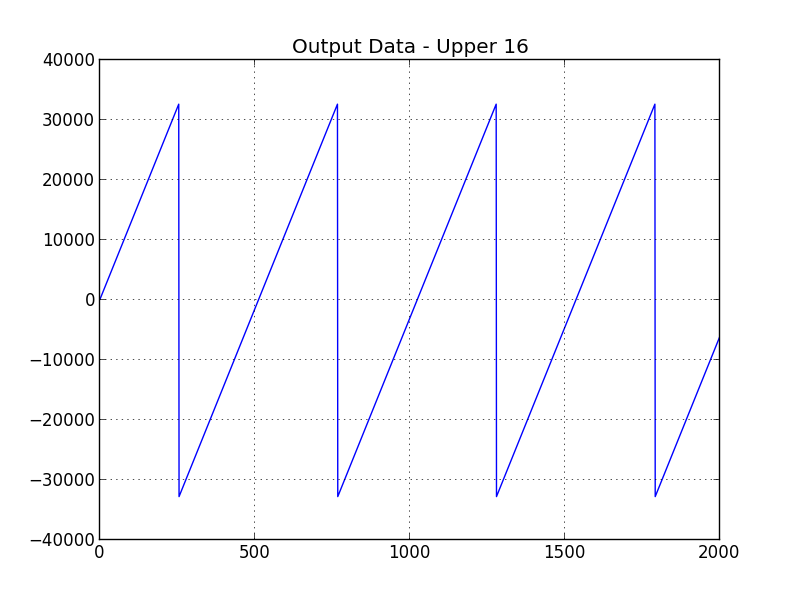
\includegraphics[scale=0.5]{./figures/upper16.jpg}
                \caption{``RAMP'' Output (Passed through by ``ANDER'')}
                \label{fig:upper16}
        \end{figure}

        \begin{figure}[h]
                \centering
                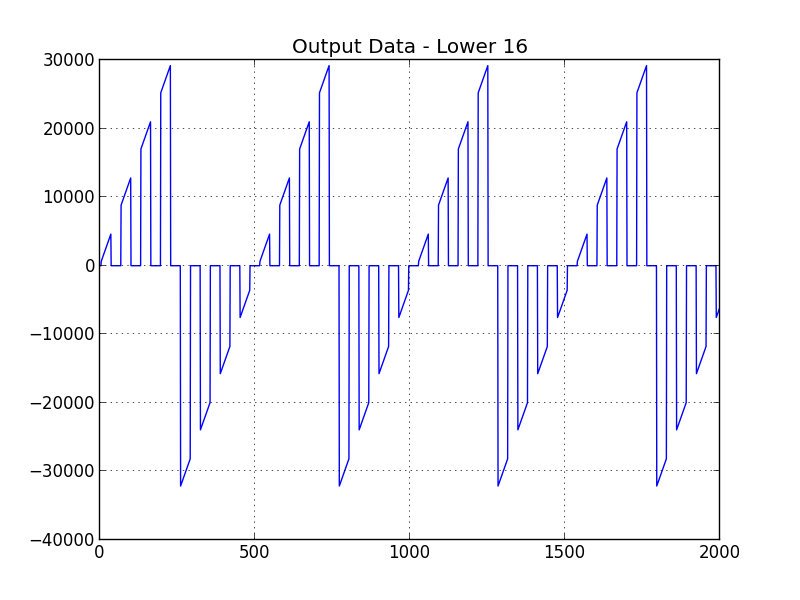
\includegraphics[scale=0.5]{./figures/lower16.jpg}
                \caption{``ANDER'' Output}
                \label{fig:lower16}
        \end{figure}

For completeness, the output plot of the \verb+square+ \textit{component} is provided in Figure \ref{fig:square_pulse}. The steps to generate a unit test for the \verb+square+ \textit{component} are outside the scope of this document.

        \begin{figure}[h]
                \centering
                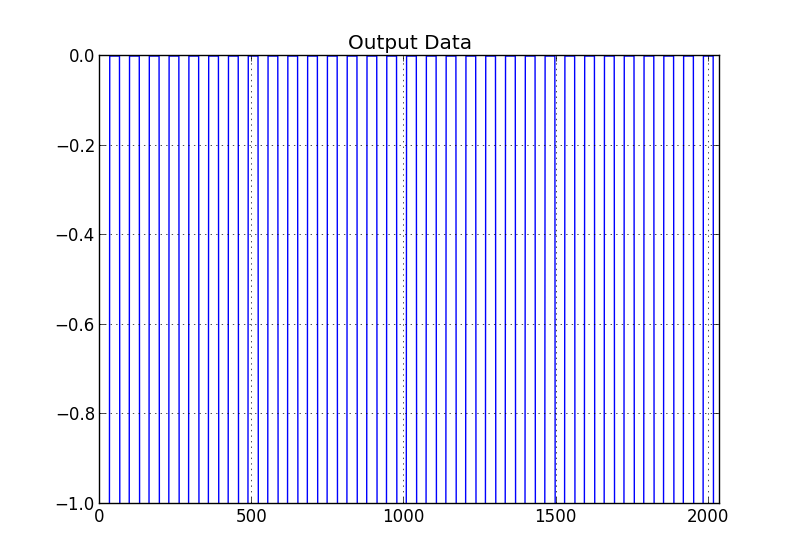
\includegraphics[scale=0.5]{./figures/square_pulse.jpg}
                \caption{``SQUARE'' Output = Input 2 to ``ANDER''}
                \label{fig:square_pulse}
        \end{figure}

%\todo{recap what was learned as a closing}

\end{document}
